
\فصل{پروتکل پیشنهادی}

در این فصل به ارائه‌ی پروتکل پیشنهادی خود برای مسیریابی در شبکه‌های مبتنی بر داده‌های نام‌گذاری شده می‌پردازیم. لازم به ذکر است همان‌طور که پیش‌تر در توضیح دامنه‌ی ارسال مسیریاب‌های NDN به آن اشاره شد، به دلیل انعطاف‌پذیر بودن و پشتیبانی از چندمسیری در این دامنه‌، بسیاری از مشکلات پیش آمده در تحویل بسته‌ها در همین دامنه مدیریت می‌شود و در نتیجه بخشی از انتظارات از قسمت مسیریابی برداشته می‌شود. به عنوان مثال اطمینان از ایجاد نشدن حلقه در مسیرها از مهم‌ترین ویژگی‌های یک پروتکل مسیریابی در شبکه‌های مبتنی بر IP می‌باشد،در حالی که به دلیل معماری NDN در دامنه‌ی ارسال از ایجاد حلقه جلوگیری می‌شود و این مسئله دیگر در نیازمندی‌های دامنه‌ی مسیریابی نیست. 

 با توجه به ساختار شبکه‌های NDN، هر پروتکلی که بخواهد روی این شبکه اجرا شود باید به چهار سوال مهم در مورد موضوعات زیر پاسخ دهد:
\شروع{فقرات}
\فقره \مهم{نام‌گذاری}: چگونگی نام‌گذاری مسیریاب‌ها، پیوند‌ها، و پیغام‌های مسیریابی
\فقره \مهم{مدل اعتماد\زیرنوشت{Trust Model}}: چگونگی توزیع کلید‌های رمز مسیریاب‌ها و اطمینان از صحت آن‌ها
\فقره \مهم{انتشار اطلاعات}: چگونگی انتشار پیغام‌های به‌روزرسانی مسیریابی در سرتاسر شبکه
\فقره \مهم{چندمسیری}: چگونگی پیدا کردن مسیرهای مختلف به یک پیشوند و رتبه‌بندی آن‌ها برای پشتبانی از چندمسیری
\پایان{فقرات}

در ادامه، از میان چهار موضوع بالا، در مورد نام‌گذاری، نحوه‌ی انتشار اطلاعات، و پشتیبانی از چندمسیری در پروتکل پیشنهادی خود صحبت خواهیم کرد. طراحی مدل اعتماد به دلیل نیاز به  پیش‌نیازهایی فراوان به آینده موکول خوهد شد. هم‌چنین در مورد پروتکل Sync و تغییریافته‌ی آن، و نیز مسئله‌ی شمارش بی‌انتها\زیرنوشت{Count to Infinity Problem} توضیح خواهیم داد.

\قسمت{نام‌گذاری}

یکی از بخش‌های مهم در پروتکل مسیریابی، تعیین نام‌گذاری مسیریاب‌ها و پیغام‌هاست. از آن جایی که مبنای شبکه‌های NDN داده‌های نام‌گذاری شده است، اگر یک پروتکل مسیریابی بخواهد به طور مستقیم روی این شبکه‌ها اجرا شود نیازمند مکانیزم نام‌گذاری متناسب با آن‌هاست. در این بخش به توضیح نام‌گذاری مسیریاب‌ها و پیشوند پیغام‌ها می‌پردازیم و نحوه‌ی نام‌گذاری دقیق‌تر پیغام‌ها را در بخش بعدی بررسی خواهیم کرد. 

با توجه به ساختار سلسله‌مراتبی شبکه، به نظر می‌رسد نام‌گذاری سلسله‌مراتبی مناسب‌ترین گزینه برای بیان ارتباط بین مولفه‌های مختلف آن باشد. بدین منظور برای هر شبکه و هر مسیریاب یک نام در نظر می‌گیریم و کافی است که نام شبکه‌ها و نیز نام مسیریاب‌ها در هر شبکه یکتا باشند. در آن صورت می‌توانیم یک مسیریاب را با نام سلسله‌مراتبی \کج{ /<network>/<router>} بشناسیم که در آن \کج{<network>} نام شبکه و \کج{<router>} نام مسیریاب است. به عنوان مثال نام یک مسیریاب در دانشگاه شریف می‌تواند \کج{/sharif/ce-router} باشد. 

در مورد نام‌گذاری پیغام‌ها باید به این نکته توجه کرد که استفاده از مخزن CCNx مستلزم این است که نام داده‌های یک مجموعه در پیشوندی که نام مجموعه است مشترک باشند. به همین دلیل برای تمام بسته‌های مربوط به مسیریابی از پیشوند \کج{/<network>/RM} استفاده می‌کنیم که در آن \کج{<network>} نام شبکه است و \کج{RM} مخفف Routing Message و برای متمایز کردن بسته‌های مسیریابی از سایر بسته‌هاست. در ادامه‌ی نام هر بسته نوع آن، نام مسیریاب تولید کننده‌ی آن، و عدد نسخه‌ی آن قرار می‌گیرند. در بخش‌های بعدی در مورد نوع بسته‌ها و نسخه‌بندی آن‌ها بیشتر توضیح خواهیم داد.

\قسمت{پیغام‌ها}

به دلیل مستقل شدن داده از مکان آن در شبکه‌های NDN، به دو نوع مسیریابی در این شبکه‌ها نیازمندیم، یک نوع مسیریابی برای یافتن تولید‌کننده‌های یک پیشوند خاص، و نوع دیگری از مسیریابی برای پیدا کردن مسیرهای بین مسیریاب‌ها برای پاسخ دادن به بسته‌های درخواست. همان‌طور که در فصل  ~\ref{prevWorks} دیدیم، بعضی از پروتکل‌های پیشنهادی برای جداکردن این دو مسیریابی از معماری دو لایه استفاده کرده‌اند تا یک لایه به نگهداری و به‌روزرسانی توپولوژی شبکه بپردازد و دیگری به توزیع پیشوند‌ها. در سایر پروتکل‌ها این جداسازی، با تفکیک بسته‌های مسیریابی پرداخته‌اند تا هر نوع بسته اطلاعات مربوط به نوع مسیریابی خاصی را در شبکه توزیع کند. ما نیز راه حل دوم را پیش می‌گیریم و دو نوع بسته‌ی مسیریابی تعریف می‌کنیم. بسته‌های نوع اول در فرآیندی مشابه پروتکل‌های مبتنی بر فاصله، اطلاعات مربوط به مسیرهای بین مسیریاب‌ها را حمل می‌کنند که آن‌ها را اعلام‌کننده‌ی فاصله\زیرنوشت{Distance Announcement} (DA) می‌نامیم. بسته‌های نوع دوم حاوی اطلاعات مربوط به پیشوند‌ها و تولید‌کنندگان آن‌ها هستند که اعلام‌کننده‌ی پیشوند\زیرنوشت{Prefix Announcement} (PA) نامیده شده‌اند. 
\begin{figure}[hb!]
\centering
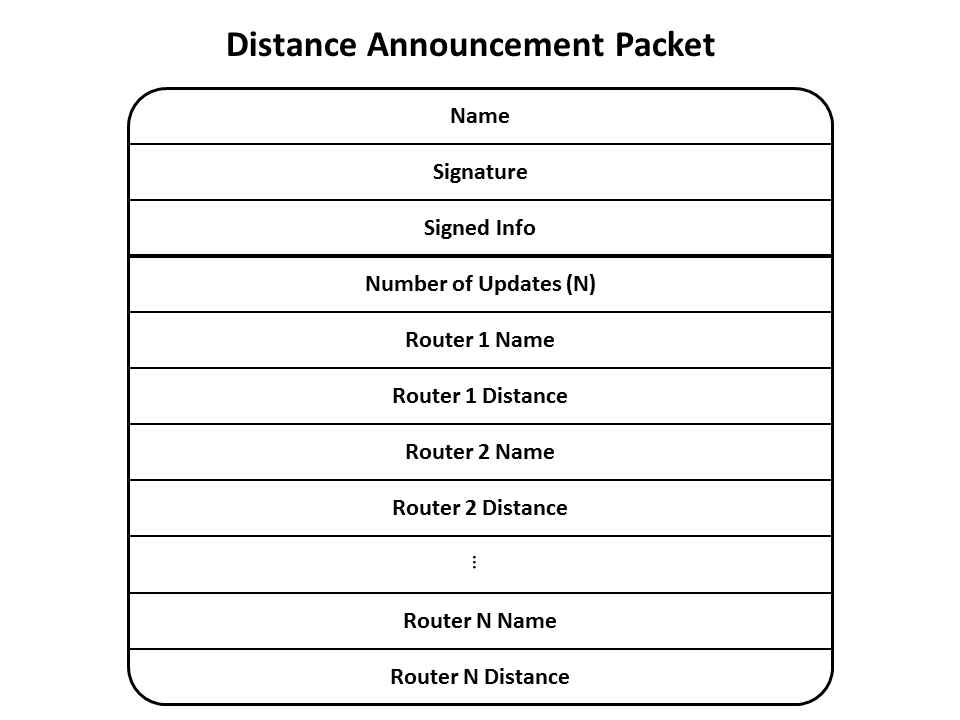
\includegraphics[scale=0.6]{./resources/figures/DA.pdf}
\caption{محتویات بسته‌ی اعلام‌کننده‌ی فاصله}
\label{fig:DA}
\end{figure}

بسته‌های DA با نام \کج{/<network>/RM/<router>/DM/<version>} مشخص می‌شوند که در آن \کج{<version>} نسخه‌ی بسته است و برای مشخص شدن آخرین به‌روزرسانی مورد استفاده قرار می‌گیرد. \کج{<router>} نام مسیریابی است که این بسته را تولید کرده است و \کج{<network>} نام شبکه‌ی آن است. محتویات این بسته را در شکل ~\ref{fig:DA} مشاهده می‌کنید. پس از سرآیند بسته‌ی داده‌ی NDN، ابتدا تعداد به روزرسانی‌ها مشخص می‌شود. سپس به ازای هر به روزرسانی نام مسیریابی که فاصله‌ی آن تغییر کرده است به همراه فاصله‌ی جدید آن قرار می‌گیرد. لازم به ذکر است که در ابتدای راه‌اندازی مسیریاب، این فاصله‌ها تنها برای همسایه‌های آن تعریف شده‌اند، و پس از دریافت پیغام‌های به روزرسانی از بقیه‌ی مسیریاب‌های شبکه، فاصله تا دیگر مسیریاب‌ها نیز مشخص می‌شوند. هم‌چنین هر مسیریاب تنها بهترین مسیرهای خود تا دیگر مسیریاب‌ها را به دیگران اعلام می‌کند. همان‌طور که در قسمت ‍~\ref{multipach} خواهیم گفت، هر مسیریاب با دریافت DA از همسایگان خود، مسیرهای متفاوت را برای مقصد‌های یکسان در نظر می‌گیرد و در FIB ذخیره می‌کند.


\begin{figure}[hb!]
\centering
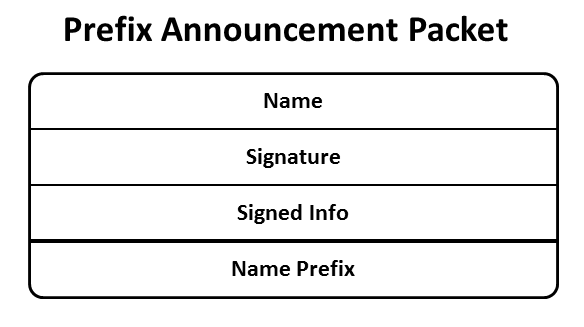
\includegraphics[scale=0.6]{./resources/figures/PA.png}
\caption{محتویات بسته‌ی اعلام‌کننده‌ی پیشوند}
\label{fig:PA}
\end{figure}

بسته‌های نوع دوم که PA نام دارند با \کج{<network>/RM/PA/<router>/ID.<ID>/<version>} مشخص می‌شوند که مشابه بسته‌های PA در آن \کج{<version>}  شماره‌ی نسخه‌ی بسته است، و \کج{<router>} و \کج{<network>} به ترتیب نام مسیریاب تولیدکننده‌ی بسته و شبکه‌ی آن هستند. محتویات این بسته را می‌توانید در شکل ~\ref{fig:PA} مشاهده کنید. در بخش داده‌ی این بسته‌ها تنها نام پیشوندنی قرار دارد که قرار است در شبکه توزیع شود یا از آن حذف شود. هر تولید‌کننده برای هر یک از پیشوند‌های خود یک بسته‌ی جدگانه با شناسه‌ی جداگانه تولید و در شبکه توزیع می‌کنند. هر مسیریاب با دریافت یکی از این بسته‌ها، با توجه به فرآیندی که در قسمت ~\ref{sync} توضیح داده خواهد شد، تشخیص می‌دهد که این پیشوند توسط تولیدکننده در اختیار قرار خواهد گرفت یا نه. در صورتی که پیشوند قابل‌دسترس باشد، اطلاعات مربوط به آن را، با استفاده از اطلاعات مسیریابی بین مسیریاب‌ها در FIB قرار می‌گیرد و در غیر این‌صورت از FIB حذف می‌شود. 


\قسمت{چندمسیری}
\label{multipach}
پیشتیبانی از چندمسیری از مهم‌ترین ویژگی‌های دامنه‌ی ارسال NDN و در نتیجه از اصلی‌ترین ویژگی‌هایی است که از یک پروتکل مسیریابی در این شبکه‌ها انتظار می‌رود. در NLSR که مبتنی بر وضعیت پیوند است و تمام مسیریاب‌ها توپولوژی شبکه را در اختیار دارند، این کار با محاسبه‌ی چند بهترین مسیر بر روی گراف شبکه انجام می‌گیرد. در این محاسبه، همه‌ی پیوندهای مسیریاب غیر از یک پیوند نادیده گرفته می‌شود و با استفاده از الگوریتم کوتاه‌ترین مسیر Dijkstra بهترین مسیر ممکن از آن پیوند و وزن آن به دست می‌آید. این کار برای تمام پیوندها تکرار می‌شود و پیوندها با توجه به وزن بهترین مسیرشان رتبه‌بندی می‌شوند و اطلاعات مربوط به آن‌ها در FIB قرار می‌گیرد. 

در پروتکل پیشنهادی ما نیازی به استفاده از الگوریتم کوتاه‌ترین مسیر نیست، زیرا هر بهترین مسیرهای هر یک از مسیریاب‌ها از طریق DA ها در اختیار مسیریاب‌های مجاورش قرار می‌گیرد و تنها کاری که مسیریاب باید انجام دهد، اجرا کردن الگوریتم مرتب‌سازی روی این مقادیر است که با توجه به تعداد کم همسایه‌ها زمان اجرای ناچیزی دارد. پس از انجام مرتب‌سازی، اطلاعات مربوط به این مسیرها در FIB  قرار خواهد گرفت.

ذکر این نکته لازم به نظر می‌رسد که اطلاعات مسیریابی درون FIB و رتبه‌بندی مسیر‌ها تنها به عنوان راهنما برای دامنه‌ی ارسال مورد استفاده قرار می‌گیرند. همان‌طور که در ?? به آن اشاره شد، دامنه‌ی ارسال در شبکه‌های NDN با نگهداری اطلاعاتی در مورد وضعیت کارایی تحویل و پاسخ به بسته‌ها روی پیوند‌های مختلف در PIT، وضعیت آن‌ها را به طور پویا مورد بررسی قرار  می‌دهد و در حقیقت از این اطلاعات برای رتبه‌بندی پیوندها استفاده می‌کند. با این حال رتبه‌بندی به دست آمده در دامنه‌ی مسیریابی هم‌چنان از اهمیت فراوانی برخوردار است و کارایی را در مورد اولین درخواست‌ها به یک داده و یا برای پیدا کردن مسیرهای جایگزین در صورت بروز مشکل در یک مسیر افزایش خواهد داد.

\قسمت{پروتکل Sync}
\label{sync}